\documentclass[12pt, a4paper]{article}

% ============================================================
%  Preamble (mirrors leak-whitepaper.tex so the two documents
%  share one toolchain: latexmk -> pdflatex + biber)
% ============================================================
\usepackage[utf8]{inputenc}
\usepackage[T1]{fontenc}
\usepackage{lmodern}
\usepackage{microtype}
\usepackage{amsmath, amssymb, amsthm}
\usepackage{graphicx}
\usepackage{booktabs}
\usepackage{array}
\usepackage{longtable}
\usepackage{listings}
\usepackage{xcolor}
\usepackage{enumitem}
\usepackage{titlesec}
\usepackage{abstract}
\usepackage{caption}
\usepackage{float}
\usepackage{pgfplots}
\pgfplotsset{compat=1.18}
\usepackage[margin=2.8cm]{geometry}
\usepackage[backend=biber, style=numeric, urldate=long]{biblatex}
\usepackage{hyperref} % load last

\addbibresource{sample.bib}
\addbibresource{benchmark-report.bib}

\hypersetup{
    colorlinks=true,
    linkcolor=blue!60!black,
    urlcolor=blue!60!black,
    citecolor=green!50!black
}

\emergencystretch=3em % long \texttt run/theorem names don't hyphenate
\titleformat{\section}{\large\bfseries}{\thesection.}{0.6em}{}
\titleformat{\subsection}{\normalsize\bfseries}{\thesubsection}{0.6em}{}

\definecolor{codebg}{HTML}{F5F5F5}
\definecolor{codekeyword}{HTML}{2E4DA0}
\lstdefinelanguage{Lean4}{
  keywords={theorem, lemma, def, let, have, intro, cases, induction, exact,
            apply, refine, rw, simp, ring, linarith, nlinarith, omega, by,
            sorry, import, open, Type, Prop},
  keywordstyle=\color{codekeyword}\bfseries,
  sensitive=true,
  comment=[l]{--},
}
\lstset{language=Lean4, backgroundcolor=\color{codebg}, basicstyle=\ttfamily\small,
        breaklines=true, frame=single, framerule=0pt, xleftmargin=6pt,
        literate={∃}{{$\exists$}}1 {∧}{{$\wedge$}}1 {→}{{$\to$}}1
                 {⊗}{{$\otimes$}}1 {⊕}{{$\oplus$}}1 {∀}{{$\forall$}}1}

% Shorthand for run labels / ids / commits
\newcommand{\run}[1]{\texttt{#1}}
\newcommand{\cmark}{$\checkmark$}

\title{\textbf{To what extent does scaffolding improve automated theorem
provers driven by large agents?}}
\author{Mikael Bashir - 02382080}
\date{14 August 2026}

\begin{document}
\maketitle

\begin{abstract}
\noindent
We report results from three benchmark runs of the Leak \cite{leakabout} automated
theorem-proving stack on FATE-X \cite{fatex2025}, a 100-problem graduate-level
abstract and commutative-algebra benchmark in Lean~4 \cite{demoura2021lean4}.The headline 
finding is negative for our central design hypothesis: on identical time budgets and the same base agent, a single
flat agent with compiler and search access (Control~II) solved
\textbf{38/98 (38.8\%)}, outperforming the best decomposition pipeline
Ultra Fleeting, \textbf{28/98, (28.6\%)}. Decomposition contributed only two problems
the flat agent could not solve. We analyse where each approach wins (\S\ref{sec:headtohead}), quantify a
difficulty cliff in FATE-X's top quartile (2/25 for both arms) (\S\ref{sec:difficulty}), mention
the events that shaped the design, including the MCP services we made
extensive use of (\S\ref{sec:verifiers}), and lay out the follow-up experiments the results motivate or
that could not be completed due to budget (\S\ref{sec:nextsteps}).
\end{abstract}

\tableofcontents
\newpage

% ============================================================
\section{Introduction}
% ============================================================

There has been extensive work on LLMs, specifically on Automated Theorem Proving systems 
driven by LLMs, with a variety of architecture designs, both in the development of the LLM itself,
and the orchestration of the LLM. We are also seeing the number of agentic systems being made publically available
increase rapidly, which raises the natural question "Do the same techniques for ATP on LLMs apply to Agentic systems, and to what extent". 
We present the Leak stack, an agentic theorem-proving system for Lean~4 + Mathlib
\cite{demoura2021lean4,mathlib2020} that tries to answer exactly this, armed with select, specialist remote verification services
(``Leak~I--XIV'') and a local bridge that drives LLM agents against them
\cite{competemath,hfspaces}. Its design bet, shared with a line of recent work
on hierarchical and decomposition-based proving
\cite{lample2022hypertree,deepseekproverv2,decomposition_openreview,davis2025goedelspoetry},
is that hard theorems are best attacked by splitting them into sub-goals proved
by parallel sub-agents. This report evaluates that bet empirically, while also 
testing if this still holds in large agentic systems such as Claude, which already have secret
scaffolding built into them \cite{anthropicharness}.

We ran several full benchmark passes on a sanitised (\S\ref{sec:benchmark}) FATE-X
\cite{fatex2025,benchmarklist_fatex}, reporting in this paper the results of 3 runs. The experiments were designed to answer three questions:

\begin{enumerate}[itemsep=1pt]
  \item \textbf{Absolute proving capacity.} What fraction of an algebra
        benchmark, exceeding PhD qualifying exam difficulty,
        can Leak close under fixed time budgets (FATE-X)?
  \item \textbf{Adding scaffolding vs.\ Relying on built-in scaffolding.} Does the lifted architecture
        (blueprint\,$\to$\,node-provers\,$\to$\,refinement) beat a
        single continuous agent given the same model and budget (and select proving tools)?
  \item \textbf{Does Sonnet 5 benefit significantly when given pantograph?} While we armed many runs
        with an improved pantograph service \cite{leakii2026upgrade},
        we always took for granted its benefit - but in the context of agentic systems, how much
        does pantograph actually buy.
\end{enumerate}

Questions 1 is objectively answered below, and we provide evidences below for questions 2 and 3.

% ============================================================
\section{Related work}
% ============================================================

Automated theorem provers are typically evaluated on miniF2F
\cite{zheng2022minif2f}, PutnamBench \cite{tsoukalas2024putnambench}, or
competition sets targeted by systems such as GPT-f \cite{polu2020gptf},
HyperTree Proof Search \cite{lample2022hypertree}, AlphaProof
\cite{alphaproof2024}, DeepSeek-Prover-V2 \cite{deepseekproverv2}, and the
G\"odel-Prover line \cite{davis2025goedelspoetry}. FATE-X \cite{fatex2025}
is deliberately harder and narrower: 100 abstract/commutative-algebra problems
drawn from graduate textbooks, qualifying exams, and research literature,
ordered by increasing difficulty. Its authors report frontier systems solving
only single-digit counts on the upper half \cite{benchmarklist_fatex}, which
matches the cliff we observe (\S\ref{sec:difficulty}), though it should be
noted that the SOTA models the authors tested with were not used as they were designed
(self-correction was disabled). \\

Decomposition-style pipelines --- sketching a proof outline and delegating
sub-goals --- descend from Draft--Sketch--Prove-like designs and are the core of
DeepSeek-Prover-V2's subgoal decomposition \cite{deepseekproverv2} and related
hierarchical searches \cite{lample2022hypertree,decomposition_openreview}. We test an already
researched and documented pipeline, Goedel-Architect \cite{goedelarchitect}, changing the driving
backbone --- instead of a fast and small LLM, such as the DeepSeek-V4-Flash backbone used by
Goedel-Architect, we drive with a large agent (Claude Sonnet~5 Agent \cite{anthropic2026sonnet5}),
referring to this design as Ultra Fleeting through out the paper;
as far as we are aware the team behind Goedel Architect have not made available the critical
scaffolding on DeepSeek-V4-Flash, so we try to replicate as closely as possible from their report.
The main features are a blueprint stage that compiles a skeleton of \texttt{sorry}-holes, 
node provers that fill holes as ReAct-style tool agents \cite{yao2023react} against live compiler service feedback, 
and a refinement stage restructures the skeleton between iterations. Contrary to the paper's suggestions, we 
deliberately omit a natural-language seed/proof, on the untested and unverified assumption 
that recent capability gains — from drivers like DeepSeek-V4-Flash to Sonnet 5 — are concentrated in reasoning 
rather than knowledge, so seeding a candidate proof should benefit a strong-reasoning driver little in a formal verification task. 
We also experiment with Pantograph \cite{aniva2024pantograph,pypantograph}, extended with a
snapshot-based ``ghost state'' model \cite{shen2026snapshot,leakii2026upgrade}
that lets many agents manage proof states on a single Lean daemon, without expensive re-elaboration. 
This service was used for Control-II runs and other experimental runs not presented in this report, 
but it wasn't used for the Ultra Fleeting benchmark, in line with the design of
the borrowed architecture. In the further-works section (\S\ref{sec:nextsteps}), we discuss some
interesting experiments that could not be completed before the writing of this report.

% ============================================================
\section{Experimental setup}
% ============================================================

\subsection{Benchmark and normalization}
\label{sec:benchmark}

FATE-X contains 100 Lean files pinning Lean \texttt{v4.28.0} \cite{fatex428}.
Our ingestion (\run{build-fatex.mjs}) normalizes each item: imports and the
\texttt{namespace ProblemN} wrapper are dropped, doc comments become the
informal statement, \texttt{section} scoping is kept, and the 38 problems with
supporting declarations get their declarations compressed into the theorem statement 
(so that problems are in the shape our harness expects). Problems are enqueued
in the benchmark's own difficulty order, so the item index doubles as a
difficulty rank. Two statements (\run{fatex\_009}, \run{fatex\_041}) do not
elaborate under our newer toolchains and were excluded from the full passes,
leaving $n=98$.

\subsection{Verification infrastructure}
\label{sec:verifiers}

All scoring is by independent re-verification, never by agent self-report.
Two verifier groups were in play, and they differ by toolchain:

\begin{itemize}[itemsep=1pt]
  \item \textbf{Leak~IV group} (Lean + Mathlib \texttt{v4.29.1}): gates every
        control run. A daemon compiles a submitted script, and a proof is only ever
        declared valid if Leak-IV returns no errors or warnings (a proof containing a sorry
        will be caught by our harness), AND the script passes strict
        regex checks to ensure the same theorem was proven (again enforced by our harness).
  \item \textbf{Leak~XI/XII/XIV group} (Lean + Mathlib \texttt{v4.32.0}):
        serves the architect pipelines (Ultra) --- XII compiles and
        elaborates a proposed blueprint/refinement, XIV verifies full scripts like IV, and XI provides Loogle/Moogle-style
        search \cite{loogle,moogle} like I.
\end{itemize}

\noindent
We have two families of services because of toolchain differences between some of the libraries involved (pantograph and lean architect).
It should not be difficult to unify the two families to run on one toolchain, but we opted to keep them seperate and
focus on the experiments instead, since our experiments did not require pantograph and architect at the same time. 
All services follow the MCP protocol on SSE transport \cite{anthropic2024mcp} (future work should consider using Streamable HTTP).

\subsection{Strategies}
\label{sec:strategies}

\begin{description}[itemsep=2pt]

  \item It is important to make clear that all of our strategy designs had their internet search tool stripped (from Claude's default tool set), so that
      we could focus on proving capacity, not retrieval capacity. Of course for formal verification, one must be familiar
      with the syntax, and thus we make available a verbose compiler daemon and toolchain pinned library search tools.
  \item[Ultra (Lifted Goedel Architect).] An inspired pipeline driven by a local
        Claude Sonnet 5 CLI \cite{anthropic2026sonnet5} instance; \run{ultra-fleeting} has no recollection
        of proved lemmas between two seperate proof attempts and was not given NL proofs to shape decomposition.
  \item[Control~II (compiler + lemma search).] Same driving agent as Ultra, armed with only Leak~IV (whole-script
        verification) and Leak~I (Loogle/Moogle lemma search
        \cite{loogle,moogle}); exactly how those tools are used is left to
        Claude's built-in harness \cite{anthropicharness}. Control-II gets no further scaffolding - benchmarked as
        \run{control-oneshot-2}. Every control run is allowed built-in Claude Code tools, such as bash, read, write, except internet search.
  \item[Control~III (blind prover).] Same driving agent as Ultra, given \emph{no} additional Leak tools:
        it is repeatedly asked to prove the target theorem and told only whether
        each attempt was correct --- never an error message --- with no context
        beyond its own previous attempts and the attempt number. A deterministic
        Leak~IV gate decides correctness. Benchmarked as \run{control-oneshot-3}.
  \item[Control~IV (compiler + pantograph + lemma search).] The same base agent armed with
        every Leak service below the X series (Leak~I--IX), again leaving all
        tool orchestration to Claude's built-in harness \cite{anthropicharness}.
        Enqueued but not yet complete at the time of writing.
\end{description}

\subsection{Protocol}
\label{sec:protocol}

One problem per worker; every attempt is bounded by wall clock only --- no
per-call caps. Budgets grew as the campaign matured: 20\,min for the first
probes (28--29~July), 30\,min mid-campaign, and 60\,min for the two full passes
and all later runs. Architect arms additionally carry
a refinement-iteration budget (5 for \run{river-vintage}, whose per-attempt
cutoff is already halved by the watcher variant; 8 for every other architect
arm).

Failure triage distinguishes infrastructure failures from problem failures:
catastrophic errors (quota, bridge down) pause the pass and \emph{release} the
claim without burning an attempt; problem-specific errors retry once, then mark
the item \emph{skipped}, which excludes it from the denominator rather than
counting as a miss. A watchdog aborts streams wedged 5 minutes past the
bridge's own deadline --- a stuck-socket backstop, not a prover cap. Every
finished attempt files a research row (tagged
\run{benchmark:fatex:<runId>}) into the same tables as production runs,
with full per-attempt metrics.

\subsection{Metrics}

Pass rate is $\text{proved}/\text{scored}$, where scored $=$ proved $+$
unsolved $+$ refuted (skipped excluded). Costs are the CLI-reported
\texttt{total\_cost\_usd} summed per item; for Claude-driver runs this is a
\emph{notional API-equivalent} figure (the operator runs on a flat-rate
subscription), while Grok-driver costs are real API spend. Times are
per-item wall clock from claim to scoring.

% ============================================================
\section{Head-to-head: decomposition vs.\ the flat agent}
\label{sec:headtohead}
% ============================================================

The campaign's central comparison is \run{LUF-Anonymous} (Ultra Fleeting:
blueprint $\to$ parallel node provers $\to$ refinement) against
\run{LC-II-Irrationality} (Control~II: one continuous agent with verifier +
search, no decomposition). Both ran claude-sonnet-5
\cite{anthropic2026sonnet5}, 60-minute budgets, over the same 98 items.

\begin{table}[H]
\centering\small
\caption{Full-pass comparison. Solve time is over proved items only.}
\label{tab:headtohead}
\begin{tabular}{@{}lrr@{}}
\toprule
 & Ultra Fleeting & Control II \\
\midrule
Proved / scored          & 28 / 98 & \textbf{38 / 98} \\
Pass rate                & 28.6\% & \textbf{38.8\%} \\
Solved by this arm only  & 2 & 12 \\
Mean (median) solve time & \textbf{827\,s} (562\,s) & 1{,}395\,s (1{,}218\,s) \\
Mean attempts per scored item & 1.24 & 1.63 \\
Median tool calls / item      & 163 & 110 \\
Median LLM calls / item       & 233 & 212 \\
Notional cost                 & \$825.53 & \$878.57 \\
Notional cost per solve       & \$29.48 & \textbf{\$23.12} \\
Verifier toolchain            & v4.32.0 & v4.29.1 \\
\bottomrule
\end{tabular}
\end{table}

\begin{figure}[H]
\centering
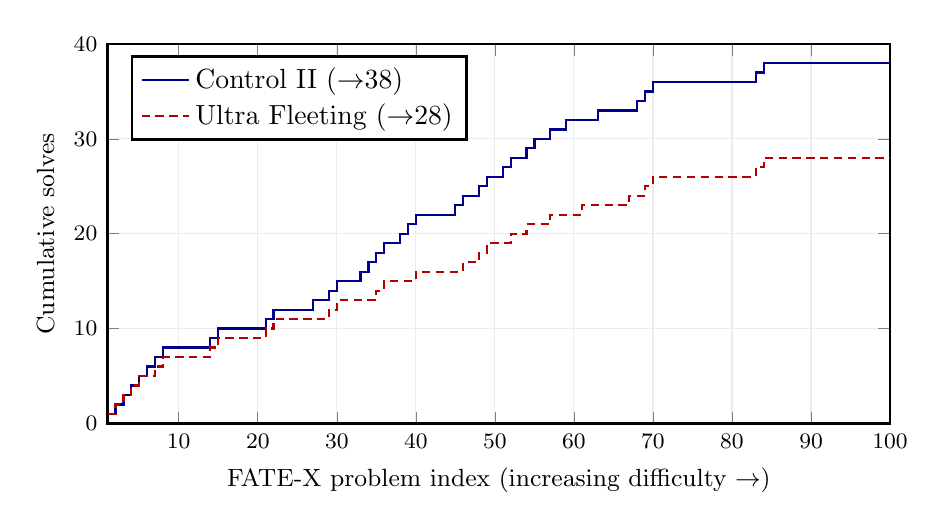
\begin{tikzpicture}
\begin{axis}[
  width=0.95\linewidth, height=6.4cm,
  xlabel={FATE-X problem index (increasing difficulty $\rightarrow$)},
  ylabel={Cumulative solves},
  xmin=1, xmax=100, ymin=0, ymax=40,
  legend pos=north west, legend cell align=left,
  grid=both, grid style={gray!15},
  tick label style={font=\footnotesize}, label style={font=\small}, thick]
\addplot[const plot, blue!55!black] coordinates {(1,1) (2,2) (3,3) (4,4) (5,5) (6,6) (7,7) (8,8) (10,8) (11,8) (12,8) (13,8) (14,9) (15,10) (16,10) (17,10) (18,10) (19,10) (20,10) (21,11) (22,12) (23,12) (24,12) (25,12) (26,12) (27,13) (28,13) (29,14) (30,15) (31,15) (32,15) (33,16) (34,17) (35,18) (36,19) (37,19) (38,20) (39,21) (40,22) (42,22) (43,22) (44,22) (45,23) (46,24) (47,24) (48,25) (49,26) (50,26) (51,27) (52,28) (53,28) (54,29) (55,30) (56,30) (57,31) (58,31) (59,32) (60,32) (61,32) (62,32) (63,33) (64,33) (65,33) (66,33) (67,33) (68,34) (69,35) (70,36) (71,36) (72,36) (73,36) (74,36) (75,36) (76,36) (77,36) (78,36) (79,36) (80,36) (81,36) (82,36) (83,37) (84,38) (85,38) (90,38) (95,38) (100,38)};
\addlegendentry{Control~II ($\rightarrow$38)}
\addplot[const plot, red!70!black, densely dashed] coordinates {(1,1) (2,2) (3,3) (4,4) (5,5) (6,5) (7,6) (8,7) (10,7) (11,7) (12,7) (13,7) (14,8) (15,9) (16,9) (17,9) (18,9) (19,9) (20,9) (21,10) (22,11) (23,11) (24,11) (25,11) (26,11) (27,11) (28,11) (29,12) (30,13) (31,13) (32,13) (33,13) (34,13) (35,14) (36,15) (37,15) (38,15) (39,15) (40,16) (42,16) (43,16) (44,16) (45,16) (46,17) (47,17) (48,18) (49,19) (50,19) (51,19) (52,20) (53,20) (54,21) (55,21) (56,21) (57,22) (58,22) (59,22) (60,22) (61,23) (62,23) (63,23) (64,23) (65,23) (66,23) (67,24) (68,24) (69,25) (70,26) (71,26) (75,26) (80,26) (82,26) (83,27) (84,28) (85,28) (90,28) (95,28) (100,28)};
\addlegendentry{Ultra Fleeting ($\rightarrow$28)}
\end{axis}
\end{tikzpicture}
\caption{Cumulative solves against difficulty rank. The two arms track each
other through the easy items, then Control~II pulls steadily ahead across the
middle third; both curves flatten after item~84 --- the difficulty cliff that
neither architecture crosses (\S\ref{sec:difficulty}).}
\label{fig:cumulative}
\end{figure}

\subsection{Agreement and discordance}

The two arms agree on 26 solves. Control~II additionally solved 12 problems
Ultra could not (\run{fatex\_006}, \run{027}, \run{033}, \run{034},
\run{038}, \run{039}, \run{045}, \run{051}, \run{055}, \run{059}, \run{063},
\run{068}); Ultra's unique contribution was 2 (\run{fatex\_061},
\run{fatex\_067}). Treating the 14 discordant problems as Bernoulli trials, an
exact two-sided sign test gives $p = 212/2^{14} \approx 0.013$: the gap is
unlikely to be noise, despite $n=1$ passes per arm.

\subsection{Interpretation}

Three observations qualify the headline number rather than reverse it:

\begin{enumerate}[itemsep=2pt]
\item \textbf{When decomposition works, it is fast.} Ultra's median solve took
      562\,s against Control~II's 1{,}218\,s --- parallel node-filling
      genuinely buys wall-clock speed on problems whose blueprints are right.
      Its per-run internals (median 6 nodes, 4 solved, 1 forfeited;
      median 2 blueprint iterations) show most solved problems needed only
      shallow decomposition.
\item \textbf{The failure mode is the blueprint, not the nodes.} On Ultra's
      70 misses the pipeline pays a fixed planning tax before any node prover
      runs, and a wrong skeleton caps what node provers can achieve. The flat
      agent spends the same minutes probing the compiler directly
      \cite{yao2023react}, and its higher attempt count (1.63 vs.\ 1.24)
      shows the budget being recycled into fresh whole-proof attempts ---
      which FATE-X's mid-range apparently rewards.
\item \textbf{Both arms die on the same wall.} In the top quartile the two
      arms converge (2/25 each, identical problems), so the architecture
      choice matters in the middle of the difficulty range, not at the top
      (\S\ref{sec:difficulty}).
\end{enumerate}

Some FATE-X items are ``flat-solvable but decomposition-hostile'': on
\run{fatex\_003} (a finite-index coset-representative theorem) both full passes
succeeded, yet a proof forced through an up-front skeleton of \texttt{have}-holes
creates sub-goals harder than the original (\S\ref{sec:fatex003}) --- a concrete
case where committing to structure early costs rather than helps.

\subsection{Difficulty gradient}
\label{sec:difficulty}

\begin{figure}[H]
\centering
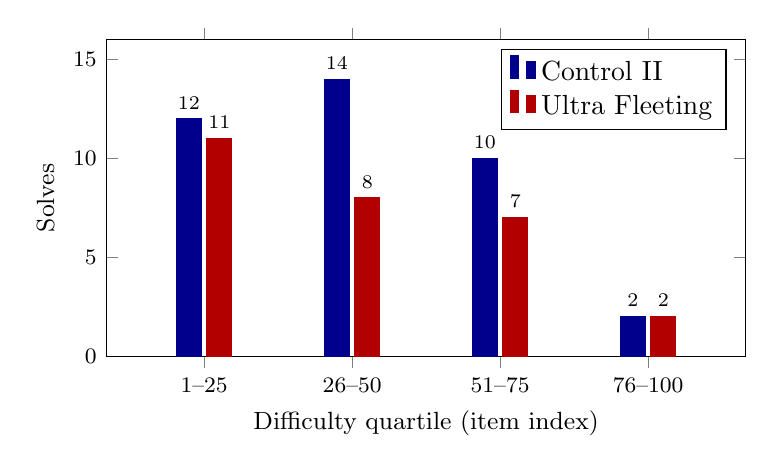
\begin{tikzpicture}
\begin{axis}[
  width=0.8\linewidth, height=5.6cm, ybar, bar width=9pt,
  xlabel={Difficulty quartile (item index)}, ylabel={Solves},
  symbolic x coords={1--25,26--50,51--75,76--100}, xtick=data,
  ymin=0, ymax=16, legend pos=north east, legend cell align=left,
  enlarge x limits=0.22, nodes near coords,
  every node near coord/.append style={font=\scriptsize},
  tick label style={font=\footnotesize}, label style={font=\small}]
\addplot[draw=blue!55!black, fill=blue!55!black] coordinates {(1--25,12) (26--50,14) (51--75,10) (76--100,2)};
\addplot[draw=red!70!black, fill=red!70!black] coordinates {(1--25,11) (26--50,8) (51--75,7) (76--100,2)};
\legend{Control~II, Ultra Fleeting}
\end{axis}
\end{tikzpicture}
\caption{Solves by FATE-X difficulty quartile (24--25 scored items each; the
benchmark is ordered by increasing difficulty \cite{fatex2025}). Control~II's
entire margin is the two middle bands; in the hardest quartile both arms solve
the same two problems.}
\label{fig:bands}
\end{figure}

Control~II's entire margin comes from the middle bands (26--75: 24 vs.\ 15).
The hardest-quartile solves are the same two problems for both arms
(\run{fatex\_083}, \run{fatex\_084}), consistent with external reports that
frontier provers solve single digits on upper FATE-X
\cite{benchmarklist_fatex}. Whatever separates items 76--100 from the rest, it
is not addressed by either architecture at a 60-minute budget.

\subsection{Solves by topic area}
\label{sec:topics}

FATE-X tags every item with a topic \cite{fatex2025}. Table~\ref{tab:topics}
breaks the two full passes down by the benchmark's own finest tag (topics with
$n\ge4$ scored items shown; the remainder are in
Appendix~\ref{app:items}).

\begin{table}[H]
\centering\small
\caption{Solves by FATE-X topic tag, both full passes.}
\label{tab:topics}
\begin{tabular}{@{}lrrr@{}}
\toprule
Topic & Scored & Ultra & Control II \\
\midrule
Localization and Decomposition of Ideals & 18 & 1 & 1 \\
Galois theory & 10 & 4 & 4 \\
Ideals and Modules & 8 & 3 & 5 \\
Integral Dependence and the Nullstellensatz & 7 & 2 & 3 \\
Tensor Product and Flatness & 7 & 0 & 2 \\
Depth, Cohen--Macaulay and Gorenstein rings & 7 & 1 & 2 \\
Heights and Dimensions & 6 & 3 & 2 \\
Group Actions and Sylow theorems & 5 & 3 & 4 \\
Regular Sequences and Regular Local Rings & 4 & 3 & 3 \\
Algebraic and Arithmetic Dynamics & 4 & 1 & 1 \\
\bottomrule
\end{tabular}
\end{table}

Two structural facts emerge. First, the benchmark's largest topic ---
localization and primary decomposition, 18 items --- is nearly untouched by
both arms (1/18 each): this single topic accounts for over a quarter of all
misses and is where FATE-X's difficulty actually lives for us, more so than
the nominal difficulty rank. Second, Control~II's margin is \emph{broad},
not deep: $+2$ on Ideals and Modules, $+2$ on Tensor/Flatness, $+1$ across
four further topics --- there is no single subject the flat agent
``understands'' better, which is consistent with its advantage being
mechanical (more whole-proof attempts per hour, \S\ref{sec:headtohead})
rather than mathematical. Ultra's only topic-level win is Heights and
Dimensions ($3$ vs.\ $2$), the home of both of its unique solves
(\S\ref{sec:cases}).

% ============================================================
\section{Case studies}
\label{sec:cases}
% ============================================================

\subsection{\run{fatex\_003}: flat-solvable, decomposition-hostile}
\label{sec:fatex003}

The clearest single-problem signal in the campaign:

\begin{lstlisting}
theorem exists_leftCoset_rightCoset_representative
    (G : Type) [Group G] (H : Subgroup G) [H.FiniteIndex] :
    ∃ S : Set G, Subgroup.IsComplement S H ∧ Subgroup.IsComplement H S := by
  sorry
\end{lstlisting}

\noindent
(``A finite-index subgroup admits a common system of representatives for its
left and right cosets.'') Both full passes solved it --- Control~II and Ultra's
whole-pipeline pass. The proof is a known short argument via Hall's
theorem-style matching already latent in Mathlib \cite{mathlib2020}; what it
punishes is \emph{premature structure}: a skeleton that commits to
constructing $S$ piecewise creates holes harder than the original goal.
Ultra survives it because its blueprint stage may emit a near-trivial
skeleton and otherwise fall back to a whole-proof attempt. This is the concrete
instance behind the ``decomposition-hostile'' label used in this report.

\subsection{\run{fatex\_061} and \run{fatex\_067}: where decomposition wins}

Ultra's two unique solves are topical neighbours (both tagged Heights and
Dimensions):
\begin{center}\small
\run{formallySmooth\_of\_formallySmooth\_quotient}\\
\run{isEmpty\_mvPowerSeries\_tensor\_mvPowerSeries\_algEquiv}
\end{center}
\noindent
--- formal smoothness descends along a square-zero quotient, and there is no
$k$-algebra isomorphism $k[[x]] \otimes_k k[[y]] \cong k[[x,y]]$. Both have
natural lemma decompositions --- an ideal-power calculation and a
cardinality/completeness obstruction respectively --- and both defeated the
flat agent's iterate-against-the-compiler style within budget. They are the
existence proof that the architect pipeline adds \emph{some} capability;
the finding of \S\ref{sec:headtohead} is that this capability is currently
narrow (2 problems) relative to its planning tax (10 problems).

\subsection{\run{fatex\_083} and \run{fatex\_084}: the only top-quartile solves}

Both arms' hardest-band solves are the same pair:
\begin{center}\small
\run{IsRegularLocalRing.flat\_local\_of\_regular}\\
\run{exists\_directSum\_free\_free\_of\_projective}
\end{center}
\noindent
--- regularity descends along a flat local homomorphism, and Eilenberg's
swindle (for projective $M$ there is a free $N$ with $M \oplus N$ free). Both are
textbook-named theorems whose informal proofs are certainly in the training
distribution \cite{anthropic2026sonnet5}, and both have short Mathlib-adjacent
formal skeletons. That the \emph{same} two problems fall to two very
different architectures suggests the top quartile is currently gated by
statement-level familiarity, not by search strategy --- consistent with the
contamination caveat of \S\ref{sec:validity} and with the flat difficulty
profile both arms show above item 76.

% ============================================================
\section{The base agent alone (Control III)}
% ============================================================

A third full pass, \run{LC-III-Await} (Leak Control III), strips the agent to
nothing: Claude Sonnet~5 is asked for a complete proof and told only whether
each attempt passed a deterministic Leak~IV gate --- no error text, no search,
no compiler feedback --- carrying forward only its own past attempts and the
attempt number. Over 42 scored items it proved \textbf{1} (\run{fatex\_002}).
We report it only in passing: the single thing it establishes is that the base
agent, unaided, cannot make headway on FATE-X --- the capability in the other
two arms comes from tool access and whole-proof iteration, not raw model
recall. No per-item obstacle was recorded, so we make no claim about \emph{why}
beyond the absence of tools and feedback.

% ============================================================
\section{Cost analysis}
\label{sec:cost}
% ============================================================

The two full passes cost \$825.53 (Ultra Fleeting) and \$878.57 (Control~II) in
CLI-reported \texttt{total\_cost\_usd}. These are \emph{notional}
API-equivalents --- the runs were driven on Claude's Max plan (20$\times$ usage
gave comfortable headroom for parallel benchmarking), not metered API spend ---
so they measure compute intensity, not cash.

On that measure the flat agent is both cheaper per solve (\$23.12 vs.\ \$29.48)
\emph{and} more capable, so on FATE-X there is no cost--quality trade-off to
argue about: Control~II dominates on both axes.

Where the compute goes is the more useful signal. A failed item is not a cheap
early exit --- it thrashes against the compiler for the full budget, costing
3--4$\times$ the tool calls of a solved item in both arms
(Fig.~\ref{fig:thrash}). Ultra's 70 misses alone are ${\sim}70$ budget-hours for
zero score. Cheap early rejection of unpromising problems is therefore the
highest-leverage efficiency work this comparison points to.

\begin{figure}[H]
\centering
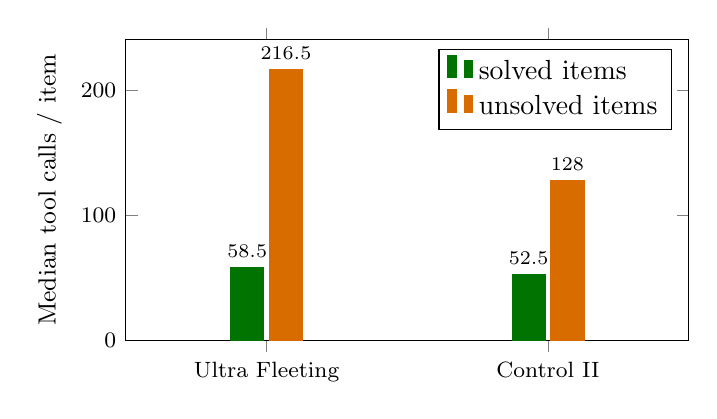
\begin{tikzpicture}
\begin{axis}[
  width=0.72\linewidth, height=5.4cm, ybar, bar width=12pt,
  ylabel={Median tool calls / item},
  symbolic x coords={Ultra Fleeting,Control II}, xtick=data,
  ymin=0, ymax=240, legend pos=north east, legend cell align=left,
  enlarge x limits=0.5, nodes near coords,
  every node near coord/.append style={font=\scriptsize},
  tick label style={font=\footnotesize}, label style={font=\small}]
\addplot[draw=green!45!black, fill=green!45!black] coordinates {(Ultra Fleeting,58.5) (Control II,52.5)};
\addplot[draw=orange!85!black, fill=orange!85!black] coordinates {(Ultra Fleeting,216.5) (Control II,128)};
\legend{solved items, unsolved items}
\end{axis}
\end{tikzpicture}
\caption{Where the compute goes: an \emph{unsolved} item costs 3--4$\times$ the
tool calls of a solved one in both arms. Failures thrash against the compiler
for the full budget rather than exiting early, which is why misses dominate
spend.}
\label{fig:thrash}
\end{figure}

% ============================================================
\section{Operational incidents and data integrity}
\label{sec:incidents}
% ============================================================

A benchmark is only as good as its bookkeeping. Three incidents from this
campaign shaped the protocol and are documented here for reproducibility:

\begin{enumerate}[itemsep=2pt]
\item \textbf{Resume-path data loss (found 8~Aug, fixed commit
      \run{f20f130}).} The console's ``from here'' requeue reset every
      non-running item at/after the target to \emph{pending} --- including
      already-scored ones. Because requeue paths never null the stored
      proof/metrics columns, the 19 wiped items of \run{LUF-Anonymous}
      (\run{fatex\_071}--\run{089}: 2 proved, 17 unsolved) were recovered by
      restoring status from the preserved columns, after a full-run JSON
      backup. The fix restricts tail-requeue to pending/skipped items; the
      \run{LUF-Anonymous} figures throughout this report are post-recovery.
\item \textbf{Certificate wipe on failed re-verification (fixed).} A failed
      re-verify of an already-proven problem could clear its stored
      certificate before staging the new result, destroying a verified proof
      on infrastructure flake. Re-verification now stages before it clears.
\item \textbf{Verifier schema mismatch.} Leak~IV's verify endpoint takes
      \run{\{script\}} while Leak~XIV takes \run{\{code,\dots\}}; mis-wiring
      surfaces as what looks like a bridge bug and, worse, as a
      wrong-toolchain gate. Run manifests now log the armed verifier and
      toolchain line per run, which is how the v4.29.1/v4.32.0 split in
      \S\ref{sec:verifiers} is known rather than assumed.
\end{enumerate}

The triage rules of \S\ref{sec:protocol} (release vs.\ retry vs.\ skip) exist
because of a fourth, older failure class: infrastructure flake silently
consuming retry budget. Releasing a claim now decrements the attempt counter,
so no quota outage can burn a problem's attempts.

% ============================================================
\section{Threats to validity}
\label{sec:validity}
% ============================================================

\begin{enumerate}[itemsep=2pt]
\item \textbf{Single passes.} Each full-pass cell is $n{=}1$ per problem; the
      sign test in \S\ref{sec:headtohead} conditions on discordant pairs but
      cannot correct for run-level luck (service latency, provider load).
\item \textbf{Sanitisation.} LUF benchmark run had a pre-sanitsation round to ensure 
      theorems are in the shape LUF expects (everything compacted into one theorem signature,
      statements all elaborate), but this process was omitted for LC-II benchmark run.
      It is worth mentioning LC-II's toolchain was one minor version ahead of
      the FATE-X pin. 
\item \textbf{Toolchain confound.} Ultra verified against Mathlib
      \texttt{v4.32.0}, Control~II against \texttt{v4.29.1}
      (\S\ref{sec:verifiers}); FATE-X itself pins \texttt{v4.28.0}
      \cite{fatex2025}. Lemma renames and automation changes between Mathlib
      versions can shift item difficulty in either direction. The two
      excluded items are excluded from \emph{both} arms, so the headline
      comparison is internally consistent, but absolute rates are not
      directly comparable with the FATE-X leaderboard without further
      restrictions for fairness.
      \cite{benchmarklist_fatex}.
\item \textbf{Contamination.} FATE-X sources include textbooks and exam
      archives that plausibly appear in model training data, stated by
      the authors of the benchmark in their paper.
      \cite{anthropic2026sonnet5}; formal statements are recent, informal
      ancestors may not be. This affects absolute rates, though it should
      affect both arms symmetrically.
\item \textbf{Notional costs.} Claude-driver dollar figures are
      API-equivalent estimates, not actual spend; for the reported benchmarks,
      we used Claude's cheaper Max Plan (20x usage provided comfortable headroom for 
      parallel benchmarking).
\end{enumerate}

% ============================================================
\section{Conclusions and next steps}
\label{sec:nextsteps}
% ============================================================

On FATE-X, at current budgets, decomposition does not beat a well-tooled flat
agent: Control~II leads Ultra Fleeting 38.8\% to 28.6\% on identical budgets and
the same model ($p\approx0.013$), at lower cost per solve
(\S\ref{sec:headtohead}). Decomposition earns its keep only in speed (562\,s
vs.\ 1{,}218\,s median per solve) and on exactly two problems the flat agent
missed (\S\ref{sec:cases}). Both arms hit the same wall in the benchmark's top
quartile, and a base agent stripped of tools and feedback manages just 1/42 ---
so on this benchmark the capability comes from tool access and whole-proof
iteration, not from the decomposition scaffold.

The comparison points to these follow-ups, in priority order:

\begin{enumerate}[itemsep=2pt]
\item \textbf{Blueprint-quality gate.} Ultra's losses concentrate in planning:
      a cheap blueprint sanity check before committing node budget (cf.\
      subgoal-quality filtering in \cite{deepseekproverv2}) is the pipeline's
      most promising fix.
\item \textbf{Early rejection.} Failed items burn the full budget
      (\S\ref{sec:cost}); a cost estimator over proof-cost history that abandons
      unpromising problems early is the highest-leverage efficiency work.
\item \textbf{Toolchain-matched re-run.} Re-verify one full pass on the other
      verifier group to bound the v4.29.1/v4.32.0 confound directly.
\item \textbf{Top-quartile study.} Items 76--100 resist both architectures;
      qualitative failure analysis on \run{fatex\_085}--\run{100} should
      precede any further architecture work aimed at them.
\end{enumerate}

\newpage
\printbibliography

\newpage
\appendix
% ============================================================
\section{Per-problem results}
\label{app:items}
% ============================================================

Full-pass outcome for every FATE-X item, in the benchmark's difficulty order
\cite{fatex2025}. UF = \run{LUF-Anonymous} (Ultra Fleeting), C2 =
\run{LC-II-Irrationality} (Control~II); \cmark{} = proved, -- = unsolved
within budget. Items 9 and 41 do not elaborate under the campaign toolchains
(\S\ref{sec:benchmark}) and were excluded. Theorem names are FATE-X's own;
topics are the benchmark's finest tag.

\begingroup\footnotesize
\setlength{\tabcolsep}{4pt}
\begin{longtable}{@{}rllcc@{}}
\caption{Per-problem outcomes for the two full passes.}
\label{tab:allitems}\\
\toprule
\# & Theorem & Topic & UF & C2 \\
\midrule
\endfirsthead
\toprule
\# & Theorem & Topic & UF & C2 \\
\midrule
\endhead
\bottomrule
\endfoot
1 & \run{isPrincipalIdealRing\_of\_associated\dots} & PID, ED and UFD & \cmark & \cmark \\
2 & \run{card\_minimal\_normal\_subgroup\_le\_2} & Subgroups and Quotient g\dots & \cmark & \cmark \\
3 & \run{exists\_leftCoset\_rightCoset\_repres\dots} & Subgroups and Quotient g\dots & \cmark & \cmark \\
4 & \run{add\_one\_eq\_two\_pow\_of\_sylow\_subgro\dots} & Group Actions and Sylow \dots & \cmark & \cmark \\
5 & \run{maximal\_abelian\_normal\_subgroup\_of\dots} & p-Groups, Nilpotent Grou\dots & \cmark & \cmark \\
6 & \run{not\_isSimpleGroup\_of\_card\_eq\_396} & Group Actions and Sylow \dots & -- & \cmark \\
7 & \run{not\_isSimpleGroup\_of\_card\_eq\_1785} & Group Actions and Sylow \dots & \cmark & \cmark \\
8 & \run{quaternionAlgebra\_isomorphic\_to\_ma\dots} & Group Actions and Sylow \dots & \cmark & \cmark \\
9 & \run{sylow\_subgroup\_not\_normal\_of\_maxim\dots} & Polynomials & \multicolumn{2}{c}{excl.} \\
10 & \run{isPrincipalIdealRing\_quot\_X\_pow\_tw\dots} & Algebraic Number Theory \dots & -- & -- \\
11 & \run{not\_isomorphic\_euclideanDomain} & Basic Definitions and Ex\dots & -- & -- \\
12 & \run{isPrincipalIdealRing\_of\_quadratic\_\dots} & Integral Dependence and \dots & -- & -- \\
13 & \run{sq\_eq\_self\_of\_not\_unit} & Galois theory & -- & -- \\
14 & \run{isomorphic\_real\_of\_fractionRing\_is\dots} & Galois theory & \cmark & \cmark \\
15 & \run{exists\_swap\_stepwiseQuotient} & Galois theory & \cmark & \cmark \\
16 & \run{normalClosure\_isPExtension\_of\_isPE\dots} & Explicit Computations & -- & -- \\
17 & \run{countable\_index\_of\_maximal\_subfiel\dots} & Galois theory & -- & -- \\
18 & \run{isEmpty\_embedding\_intermediateFiel\dots} & Galois theory & -- & -- \\
19 & \run{galoisGroup\_iso\_quaternion\_group} & Algebraic Number Theory \dots & -- & -- \\
20 & \run{generated\_single\_elem\_of\_degree\_le\_p} & Galois theory & -- & -- \\
21 & \run{intermediateField\_rank\_eq\_ringChar} & Galois theory & \cmark & \cmark \\
22 & \run{finite\_algebraic\_integers\_of\_finit\dots} & Galois theory & \cmark & \cmark \\
23 & \run{ratio\_tendsto\_one\_of\_irreducible} & Galois theory & -- & -- \\
24 & \run{galoisGroup\_iso\_of\_distinct\_primes} & Galois theory & -- & -- \\
25 & \run{fixedField\_eq\_algebra\_adjoin} & Integral Dependence and \dots & -- & -- \\
26 & \run{card\_one\_or\_two\_of\_finite\_closed\_s\dots} & Integral Dependence and \dots & -- & -- \\
27 & \run{isGalois\_and\_rank\_eq\_of\_isPrimitiv\dots} & Integral Dependence and \dots & -- & \cmark \\
28 & \run{infinite\_conj\_of\_ne\_1\_absoluteGalo\dots} & Localization and Decompo\dots & -- & -- \\
29 & \run{isClosed\_zpowers\_iff\_isOfFinOrder} & Localization and Decompo\dots & \cmark & \cmark \\
30 & \run{integrallyClosedIn\_of\_complement\_m\dots} & Integral Dependence and \dots & \cmark & \cmark \\
31 & \run{UFD\_of\_ge\_5} & Localization and Decompo\dots & -- & -- \\
32 & \run{UFD\_of\_adicCompletion\_UFD} & Localization and Decompo\dots & -- & -- \\
33 & \run{isNoetherianRing\_of\_fg\_of\_isNoethe\dots} & PID, ED and UFD & -- & \cmark \\
34 & \run{powerSeries\_not\_integrallyClosed\_o\dots} & Tensor Product and Flatn\dots & -- & \cmark \\
35 & \run{noetherian\_of\_prime\_ideals\_fg} & Ideals and Modules & \cmark & \cmark \\
36 & \run{associatedPrimes\_hom\_eq\_support\_in\dots} & Integral Dependence and \dots & \cmark & \cmark \\
37 & \run{ufd\_quotDetSubOne} & Integral Dependence and \dots & -- & -- \\
38 & \run{free\_dualNumber\_and\_rank\_eq\_2} & Tensor Product and Flatn\dots & -- & \cmark \\
39 & \run{finite\_primes\_lies\_over\_of\_finite\_\dots} & Heights and Dimensions & -- & \cmark \\
40 & \run{free\_of\_rank\_iff} & Regular Sequences and Re\dots & \cmark & \cmark \\
41 & \run{isNoetherianRing\_and\_krullDim\_eq\_top} & Tensor Product and Flatn\dots & \multicolumn{2}{c}{excl.} \\
42 & \run{nonEmpty\_ringEquiv\_of\_sub\_in\_cube} & Tensor Product and Flatn\dots & -- & -- \\
43 & \run{IsRegularLocalRing.frobenius\_flat} & Ideals and Modules & -- & -- \\
44 & \run{quot\_x2\_sub\_y2\_y2\_sub\_z2\_xy\_yz\_zx\_\dots} & Completions and Hensel's\dots & -- & -- \\
45 & \run{free\_of\_free\_resolution} & Completions and Hensel's\dots & -- & \cmark \\
46 & \run{module\_flat\_iff} & Ideals and Modules & \cmark & \cmark \\
47 & \run{isEmpty\_isomorphism\_UFD\_of\_quotient} & Depth, Cohen-Macaulay Ri\dots & -- & -- \\
48 & \run{isAbsolutelyFlat\_iff\_principal\_ide\dots} & Smoothness and the Modul\dots & \cmark & \cmark \\
49 & \run{principal\_ideal\_idempotent\_iff\_fg\_\dots} & Ideals and Modules & \cmark & \cmark \\
50 & \run{isNoetherianRing\_of\_isLocalRing\_of\dots} & Tensor Product and Flatn\dots & -- & -- \\
51 & \run{adicCompletion\_faithfullyFlat\_iff} & Polynomials & -- & \cmark \\
52 & \run{generate\_unit\_ideal\_of\_quotient} & Regular Sequences and Re\dots & \cmark & \cmark \\
53 & \run{isGorensteinRing\_quot\_x2\_sub\_y2\_y2\dots} & Tensor Product and Flatn\dots & -- & -- \\
54 & \run{not\_zero\_divisor\_of\_hausdorff\_of\_d\dots} & Basic Definitions and Ex\dots & \cmark & \cmark \\
55 & \run{stablyFree\_iff\_free\_of\_not\_fg} & Ideals and Modules & -- & \cmark \\
56 & \run{projective\_of\_faithfullyFlat\_base\_\dots} & Smoothness and the Modul\dots & -- & -- \\
57 & \run{completely\_integrally\_closed\_polyn\dots} & Dedekind Domains and DVRs & \cmark & \cmark \\
58 & \run{flat\_of\_flat\_over\_quotient} & Homological Methods & -- & -- \\
59 & \run{exists\_unique\_valuation\_eq} & Polynomials & -- & \cmark \\
60 & \run{invertible\_iff\_codimension\_one} & Depth, Cohen-Macaulay Ri\dots & -- & -- \\
61 & \run{formallySmooth\_of\_formallySmooth\_q\dots} & Heights and Dimensions & \cmark & -- \\
62 & \run{adicCompletion\_equiv\_of\_smooth} & Tensor Product and Flatn\dots & -- & -- \\
63 & \run{surjection\_of\_formally\_unramified} & Ideals and Modules & -- & \cmark \\
64 & \run{homogeneous\_coordinate\_ring\_not\_is\dots} & Depth, Cohen-Macaulay Ri\dots & -- & -- \\
65 & \run{Polynomial.isGorensteinRing} & Homological Methods & -- & -- \\
66 & \run{exists\_eq\_ofList\_and\_isRegular\_of\_\dots} & Depth, Cohen-Macaulay Ri\dots & -- & -- \\
67 & \run{isEmpty\_mvPowerSeries\_tensor\_mvPow\dots} & Heights and Dimensions & \cmark & -- \\
68 & \run{localization\_jacobson\_of\_one\_lt\_ri\dots} & Depth, Cohen-Macaulay Ri\dots & -- & \cmark \\
69 & \run{IsRegularLocalRing.regularAtPrime} & Depth, Cohen-Macaulay Ri\dots & \cmark & \cmark \\
70 & \run{exists\_minimalPrime\_map\_zero} & Regular Sequences and Re\dots & \cmark & \cmark \\
71 & \run{fixedPoints\_isCohenMacaulayRing} & Regular Sequences and Re\dots & -- & -- \\
72 & \run{isCohenMacaulay\_extendScalars\_over\dots} & Completions and Hensel's\dots & -- & -- \\
73 & \run{mvPolynomial\_quotient\_isCohenMacau\dots} & Tensor Product and Flatn\dots & -- & -- \\
74 & \run{IsRegularLocalRing.gorensteinAtReg\dots} & Depth, Cohen-Macaulay Ri\dots & -- & -- \\
75 & \run{gradedAlgebra\_isCohenMacaulay\_iff\_\dots} & Ideals and Modules & -- & -- \\
76 & \run{IsCatenary.of\_noetherian\_ufd\_of\_di\dots} & Heights and Dimensions & -- & -- \\
77 & \run{infinite\_intermediate\_primes} & Ideals and Modules & -- & -- \\
78 & \run{IsCohenMacaulayLocalRing.isGorenst\dots} & Localization and Decompo\dots & -- & -- \\
79 & \run{IsLocalRing.not\_isCompleteIntersec\dots} & Group Actions and Sylow \dots & -- & -- \\
80 & \run{isCohenMacaulayRing\_of\_dimension\_t\dots} & Polynomials & -- & -- \\
81 & \run{generated\_by\_regular\_sequence\_iff} & Homological Methods & -- & -- \\
82 & \run{subring\_iso\_mvPowerSeries\_over\_DVR} & Heights and Dimensions & -- & -- \\
83 & \run{IsRegularLocalRing.flat\_local\_of\_r\dots} & Heights and Dimensions & \cmark & \cmark \\
84 & \run{exists\_directSum\_free\_free\_of\_proj\dots} & Algebraic and Arithmetic\dots & \cmark & \cmark \\
85 & \run{exist\_euclideanDomain\_not\_norm\_nat} & Algebraic and Arithmetic\dots & -- & -- \\
86 & \run{dimension\_convex} & Algebraic and Arithmetic\dots & -- & -- \\
87 & \run{exists\_polynomial\_ringEquiv\_isEmpt\dots} & Algebraic and Arithmetic\dots & -- & -- \\
88 & \run{quotient\_not\_UFD} & Localization and Decompo\dots & -- & -- \\
89 & \run{not\_isSimpleGroup\_of\_card\_eq\_336} & Localization and Decompo\dots & -- & -- \\
90 & \run{not\_finiteType\_inf\_algebraMap\_range} & Localization and Decompo\dots & -- & -- \\
91 & \run{pic\_three\_lines} & Localization and Decompo\dots & -- & -- \\
92 & \run{dimension\_sequences\_of\_one\_dimensi\dots} & Localization and Decompo\dots & -- & -- \\
93 & \run{exists\_integral\_finiteType\_not\_fin\dots} & Localization and Decompo\dots & -- & -- \\
94 & \run{zeroSet\_finite\_or\_contain\_arithmet\dots} & Localization and Decompo\dots & -- & -- \\
95 & \run{p\_map\_ne\_p} & Localization and Decompo\dots & -- & -- \\
96 & \run{ratFunc\_square\_is\_poly\_of\_orbit\_co\dots} & Localization and Decompo\dots & -- & -- \\
97 & \run{exists\_point\_not\_in\_zero\_set} & Localization and Decompo\dots & -- & -- \\
98 & \run{exists\_maximal\_ideal\_not\_in\_finite\dots} & Localization and Decompo\dots & -- & -- \\
99 & \run{equiv\_of\_aut\_equiv} & Localization and Decompo\dots & -- & -- \\
100 & \run{free\_of\_countably\_generated\_projec\dots} & Localization and Decompo\dots & -- & -- \\

\end{longtable}
\endgroup

\end{document}
